\section{随机变量的数字特征}

分布函数或密度函数把随机变量描述得很完整，但完整不等于好用。面对两个投资方案、两批零件的尺寸，我们通常只想知道“平均有多少”“波动有多大”“两个量是否同向变化”。这些数就是数字特征：它们丢掉分布的细节，把最要紧的几条信息压缩成几个实数，便于比较，也便于代入后续公式。

\subsection{期望：以概率加权的平均}

先看一个离散的例子。某抽奖活动每次的奖金 $X$（元）只能取 $0,1,2,5$ 这五个值，概率依次是 $0.2,0.3,0.4,0.1$。抽一次平均能拿多少？把每个取值乘以它出现的概率再相加：
\[
E(X)=0\times0.2+1\times0.3+2\times0.4+5\times0.1=1.6 .
\]
$1.6$ 不是某次真能拿到的金额（取值里根本没有 $1.6$），而是大量重复抽奖后平均每次的收益。重复 $n$ 次，平均奖金会随 $n$ 增大向 $1.6$ 靠拢。

一般地，若离散型随机变量 $X$ 的分布律为 $P(X=x_i)=p_i$，且
\[
\sum_i |x_i|p_i<\infty ,
\]
则称
\[
E(X)=\sum_i x_i p_i
\]
为 $X$ 的数学期望。连续型随机变量把分布律换成密度、求和换成积分。只要绝对矩有限，即
\[
\int_{-\infty}^{+\infty}|x|f(x)\,\mathrm{d}x<\infty ,
\]
就定义
\[
E(X)=\int_{-\infty}^{+\infty}x f(x)\,\mathrm{d}x .
\]
两个定义都要求绝对收敛，这不是技术上的洁癖。若级数只是条件收敛，重新排列求和次序会得到不同的值，而“平均”不应该取决于我们把取值按什么顺序排列；绝对收敛才能保证 $E(X)$ 由分布本身唯一确定。

期望也可能不存在。柯西分布的密度为 $f(x)=\dfrac{1}{\pi(1+x^2)}$，它关于原点对称，但
\[
\int_{-\infty}^{+\infty}|x|f(x)\,\mathrm{d}x=\frac{2}{\pi}\int_0^{+\infty}\frac{x}{1+x^2}\,\mathrm{d}x=+\infty ,
\]
正负两侧的“面积矩”都发散，谈不上相抵后的位置，所以柯西分布没有期望。对称性只能说明“如果期望存在，它等于 $0$”，不能保证存在。

\begin{center}
\begin{tikzpicture}
\begin{axis}[
  width=0.80\linewidth,height=5.4cm,
  ybar,bar width=15pt,
  xmin=-0.7,xmax=5.7,ymin=-0.14,ymax=0.46,
  xtick={0,1,2,5},ytick={0,0.1,0.2,0.3,0.4},
  xlabel={$x$},ylabel={$p_i$},
  axis lines=left,
  tick label style={font=\scriptsize},
  label style={font=\small},
]
\addplot[fill=blue!30,draw=blue!60!black] coordinates {(0,0.2)(1,0.3)(2,0.4)(5,0.1)};
\draw[gray!70] (axis cs:-0.7,0) -- (axis cs:5.7,0);
\fill[red!70!black] (axis cs:1.6,0) -- (axis cs:1.49,-0.10) -- (axis cs:1.71,-0.10) -- cycle;
\draw[dashed,red!70!black,thick] (axis cs:1.6,0) -- (axis cs:1.6,0.45);
\node[font=\scriptsize,red!70!black,anchor=south] at (axis cs:1.6,0.45){$E(X)=1.6$};
\node[font=\scriptsize,anchor=west] at (axis cs:1.80,-0.075){支点};
\end{axis}
\end{tikzpicture}
\par\vspace{2pt}
{\footnotesize\itshape 柱子高度是概率，柱子的“质量”落在取值 $x_i$ 上。$E(X)=1.6$ 是这组质量的重心：支点放在 $1.6$，左右力矩恰好相等，
$0.2\times1.6+0.3\times0.6=0.4\times0.4+0.1\times3.4=0.5$。最可能的取值是 $2$，但期望并不是众数——它由全部取值和概率共同决定。}
\end{center}

期望最重要的性质是线性性。对任意常数 $a,b,c$，
\[
E(aX+bY+c)=aE(X)+bE(Y)+c .
\]
这条性质不要求 $X,Y$ 独立，甚至不要求它们有联合密度：只要三个期望都存在，就把联合分布按行、按列求和，常数项按总概率 $1$ 提出来即可。

乘积则不能随便拆。$E(XY)=E(X)E(Y)$ 需要额外条件，最常用的是 $X,Y$ 相互独立：独立时 $p_{ij}=p_{i\cdot}p_{\cdot j}$，双重和可以拆成两个和的乘积。没有独立性时等式一般不成立。例如 $X$ 等可能取 $\pm1$，令 $Y=X$，则 $E(XY)=E(X^2)=1$，而 $E(X)E(Y)=0$。

已知 $X$ 的分布求 $g(X)$ 的期望时，不必先写出 $g(X)$ 的分布，直接按 $X$ 的分布加权即可：
\[
E[g(X)]=\sum_i g(x_i)p_i
\quad\text{或}\quad
E[g(X)]=\int_{-\infty}^{+\infty}g(x)f(x)\,\mathrm{d}x ,
\]
当然仍要求相应的和或积分绝对收敛。比如 $X$ 的密度为 $f(x)=2x\ (0<x<1)$，取 $g(x)=x^2$，直接算得
\[
E(X^2)=\int_0^1 x^2\cdot2x\,\mathrm{d}x=\frac12 ,
\]
而 $(E X)^2=\left(\frac23\right)^2=\frac49$。两者不相等，差值 $\frac12-\frac49=\frac1{18}$ 正是下一节的方差。

\begin{center}
\begin{tikzpicture}
\begin{axis}[
  name=dens,
  width=6.4cm,height=4.6cm,
  xmin=-0.04,xmax=1.08,ymin=0,ymax=2.3,
  xtick={0,0.5,1},ytick={0,1,2},
  xlabel={$x$},ylabel={$f(x)$},
  title={密度 $f(x)=2x$},
  title style={font=\scriptsize},
  axis lines=left,
  tick label style={font=\scriptsize},
  label style={font=\scriptsize},
]
\addplot[blue!60!black,thick,domain=0:1,samples=60] {2*x};
\end{axis}
\begin{axis}[
  at={(7.2cm,0)},anchor=south west,
  width=6.4cm,height=4.6cm,
  xmin=-0.04,xmax=1.08,ymin=0,ymax=2.3,
  xtick={0,0.5,1},ytick={0,1,2},
  xlabel={$x$},ylabel={$g(x)f(x)$},
  title={被积函数 $g(x)f(x)=2x^3$},
  title style={font=\scriptsize},
  axis lines=left,
  tick label style={font=\scriptsize},
  label style={font=\scriptsize},
]
\addplot[fill=red!18,draw=red!65!black,domain=0:1,samples=60] {2*x^3} \closedcycle;
\node[font=\scriptsize,red!65!black] at (axis cs:0.62,0.55){面积 $=\frac12$};
\end{axis}
\end{tikzpicture}
\par\vspace{2pt}
{\footnotesize\itshape 左图是 $X$ 的密度，右图把每个 $x$ 上的密度乘以 $g(x)=x^2$。右图曲线下的面积就是 $E[g(X)]=\int_0^1 2x^3\,\mathrm{d}x=\frac12$。求 $E[g(X)]$ 只需在 $x$ 轴上按密度加权，不需要先求 $g(X)$ 的密度。}
\end{center}

连续型期望常用对称性和换元。设 $Z\sim N(0,1)$，密度 $\varphi(z)=\frac{1}{\sqrt{2\pi}}\mathrm{e}^{-z^2/2}$。被积函数 $z\varphi(z)$ 是奇函数，故 $E(Z)=0$。二阶矩用分部积分，注意 $z\varphi(z)=-\varphi'(z)$：
\[
E(Z^2)=\int_{-\infty}^{+\infty}z^2\varphi(z)\,\mathrm{d}z
=-\int_{-\infty}^{+\infty}z\,\mathrm{d}\varphi(z)
=\int_{-\infty}^{+\infty}\varphi(z)\,\mathrm{d}z=1 .
\]
若 $X=\mu+\sigma Z$，由线性性立刻得到 $E(X)=\mu$；方差将在下一节由 $D(X)=\sigma^2D(Z)$ 得到。

\subsection{方差：平均偏离有多远}

期望只说明中心位置。两个方案的年化收益期望都是 $5\%$，一个每年在 $4\%$ 到 $6\%$ 之间小幅摆动，另一个可能一年赚 $20\%$、下一年亏 $10\%$，风险显然不同。刻画这种波动，最常用的是“偏离期望的平方的平均”：
\[
D(X)=E\bigl[(X-E(X))^2\bigr].
\]
它恒不为负；单位是 $X$ 的单位的平方（元$^2$、米$^2$），所以实际报告时常开方，称
\[
\sigma(X)=\sqrt{D(X)}
\]
为标准差，单位和 $X$ 一致。

方差还有一条更省事的计算公式。把平方展开：
\[
D(X)=E\bigl[X^2-2X\,E(X)+(E X)^2\bigr]
=E(X^2)-2(E X)^2+(E X)^2
=E(X^2)-(E X)^2 .
\]
实际计算几乎都用右边：先算 $E(X^2)$ 和 $E(X)$，再相减。要注意 $E(X^2)\ge(E X)^2$ 恒成立，差额就是方差。

方差还是“用常数逼近 $X$”时的最小均方误差。对任意实数 $c$，
\[
E[(X-c)^2]=E\bigl[(X-E X)+(E X-c)\bigr]^2
=D(X)+(E X-c)^2\ge D(X),
\]
等号仅在 $c=E(X)$ 时成立。所以期望是均方意义下最靠近 $X$ 的常数，方差是这个最近距离的平方。这条恒等式也是后面“条件期望是最优预测”的雏形。

\begin{center}
\begin{tikzpicture}
\begin{axis}[
  width=0.82\linewidth,height=5.4cm,
  xmin=-4,xmax=4,ymin=0,ymax=0.72,
  xtick={-2,-1,0,1,2},ytick={0,0.2,0.4,0.6},
  xlabel={$x$},ylabel={密度},
  axis lines=left,
  tick label style={font=\scriptsize},
  label style={font=\small},
  legend style={font=\scriptsize,draw=none,fill=none,at={(0.98,0.98)},anchor=north east},
]
\addplot[blue!65!black,thick,domain=-4:4,samples=200] {0.5694*exp(-x^2/(2*0.49))};
\addlegendentry{$\sigma=0.7$}
\addplot[red!65!black,thick,domain=-4:4,samples=200] {0.2216*exp(-x^2/(2*3.24))};
\addlegendentry{$\sigma=1.8$}
\draw[dashed,blue!55] (axis cs:-0.7,0) -- (axis cs:-0.7,0.36);
\draw[dashed,blue!55] (axis cs:0.7,0) -- (axis cs:0.7,0.36);
\draw[dashed,red!55] (axis cs:-1.8,0) -- (axis cs:-1.8,0.13);
\draw[dashed,red!55] (axis cs:1.8,0) -- (axis cs:1.8,0.13);


\draw[dashed,gray!60] (axis cs:0,0) -- (axis cs:0,0.60);
\node[font=\scriptsize,gray!70!black,anchor=south] at (axis cs:0,0.60){$\mu$};
\end{axis}
\end{tikzpicture}
\par\vspace{2pt}
{\footnotesize\itshape 两条正态密度都以 $0$ 为期望。蓝色 $\sigma=0.7$，红色 $\sigma=1.8$：峰值 $1/(\sigma\sqrt{2\pi})$ 与 $\sigma$ 成反比，$\sigma$ 越大曲线越矮越胖。对正态分布，约有 $68.3\%$ 的概率落在 $\mu\pm\sigma$ 内（图中虚线之间），所以 $\sigma$ 直接给出了“典型波动范围”的尺度。}
\end{center}

方差的基本性质都可由定义推出：
\begin{itemize}
  \item $D(C)=0$（常数没有波动）；反之 $D(X)=0$ 的充要条件是 $P(X=E X)=1$。因为 $(X-EX)^2$ 非负，非负随机变量期望为零只能说明它几乎处处为零。
  \item $D(aX+b)=a^2D(X)$。平移不改变相对位置，乘 $a$ 把每个偏差放大 $|a|$ 倍，平方后放大 $a^2$ 倍。
  \item 一般情形下 $D(X\pm Y)=D(X)+D(Y)\pm2\Cov(X,Y)$，其中 $\Cov$ 是下一节的协方差。只有 $X,Y$ 不相关时才能直接相加。
\end{itemize}

若 $\sigma(X)>0$，把 $X$ 平移再缩放，得到标准化随机变量
\[
X^*=\frac{X-E(X)}{\sigma(X)},
\qquad E(X^*)=0,\quad D(X^*)=1 .
\]
不同量纲的随机变量经过这一步可以放在同一把尺子上比较，$X^*$ 的取值称为 $z$ 分数。

方差还给出一个不依赖分布形状的概率界。对任意 $\varepsilon>0$，
\[
P\bigl(|X-E X|\ge\varepsilon\bigr)
\le \frac{D(X)}{\varepsilon^2},
\]
因为事件 $\{|X-EX|\ge\varepsilon\}$ 上 $(X-EX)^2\ge\varepsilon^2$，两边取期望即得。这个界通常偏松（例如正态分布在 $2\sigma$ 外的真实概率约 $0.046$，界给出 $0.25$），但它的价值在于不需要知道分布。

常见分布的期望与方差列在下表，几何分布按“首次成功所需的试验次数”（取值 $1,2,\dots$）定义。

\begin{center}
\begin{tabular}{cccc}
\toprule
分布 & 记号 & 期望 & 方差 \\
\midrule
$0$-$1$ 分布 & $B(1,p)$ & $p$ & $p(1-p)$ \\
二项分布 & $B(n,p)$ & $np$ & $np(1-p)$ \\
泊松分布 & $P(\lambda)$ & $\lambda$ & $\lambda$ \\
几何分布 & $G(p)$ & $1/p$ & $(1-p)/p^2$ \\
均匀分布 & $U(a,b)$ & $(a+b)/2$ & $(b-a)^2/12$ \\
指数分布 & $E(\lambda)$ & $1/\lambda$ & $1/\lambda^2$ \\
正态分布 & $N(\mu,\sigma^2)$ & $\mu$ & $\sigma^2$ \\
\bottomrule
\end{tabular}
\end{center}

这些结果最好按定义推一遍再记。例如指数分布 $f(x)=\lambda\mathrm{e}^{-\lambda x}\ (x>0)$，
\[
E(X)=\int_0^{\infty}x\lambda\mathrm{e}^{-\lambda x}\,\mathrm{d}x=\frac1\lambda,
\qquad
E(X^2)=\int_0^{\infty}x^2\lambda\mathrm{e}^{-\lambda x}\,\mathrm{d}x=\frac{2}{\lambda^2},
\]
故 $D(X)=\frac{2}{\lambda^2}-\frac{1}{\lambda^2}=\frac{1}{\lambda^2}$。指数分布的期望和标准差相等，都是 $1/\lambda$，这是它区别于其他连续分布的一个标志。

\subsection{协方差与相关系数}

两个随机变量放在一起时，各自的期望、方差还不够。$D(X+Y)$ 展开会出现交叉项
\[
D(X+Y)=D(X)+D(Y)+2E\bigl[(X-E X)(Y-E Y)\bigr],
\]
中间这一项刻画 $X,Y$ 是同向偏离还是反向偏离，称为协方差：
\[
\Cov(X,Y)=E\bigl[(X-E X)(Y-E Y)\bigr].
\]
展开平方同样得到常用的计算公式
\[
\Cov(X,Y)=E(XY)-E(X)E(Y).
\]
协方差的符号有直接含义：若 $X$ 高于均值时 $Y$ 也倾向于高于均值，乘积多为正，协方差为正；若一个高时另一个偏低，乘积多为负，协方差为负。

\begin{center}
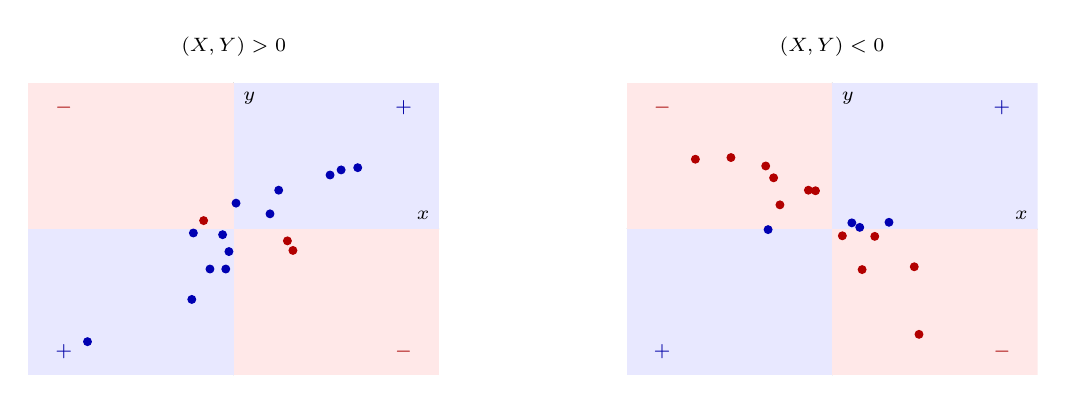
\begin{tikzpicture}
\begin{axis}[
  name=covpos,
  width=6.8cm,height=5.3cm,
  xmin=-2.6,xmax=2.6,ymin=-2.6,ymax=2.6,
  xtick=\empty,ytick=\empty,
  xlabel={$x$},ylabel={$y$},
  title={$\Cov(X,Y)>0$},
  title style={font=\scriptsize},
  axis lines=middle,
  tick label style={font=\scriptsize},
  label style={font=\scriptsize},
]
\fill[blue!9] (axis cs:0,0) rectangle (axis cs:2.6,2.6);
\fill[blue!9] (axis cs:-2.6,-2.6) rectangle (axis cs:0,0);
\fill[red!9] (axis cs:-2.6,0) rectangle (axis cs:0,2.6);
\fill[red!9] (axis cs:0,-2.6) rectangle (axis cs:2.6,0);
\node[font=\scriptsize,blue!65!black] at (axis cs:2.15,2.16){$+$};
\node[font=\scriptsize,red!65!black] at (axis cs:-2.15,2.16){$-$};
\node[font=\scriptsize,blue!65!black] at (axis cs:-2.15,-2.17){$+$};
\node[font=\scriptsize,red!65!black] at (axis cs:2.15,-2.17){$-$};
\addplot[only marks,mark=*,mark size=1.4pt,blue!70!black] coordinates {
(0.03,0.46) (1.36,1.05) (1.22,0.96) (-0.51,-0.07) (-0.30,-0.71) (-0.53,-1.25)
(0.57,0.69) (-0.06,-0.40) (-1.85,-2.00) (1.57,1.09) (-0.10,-0.71)
(-0.14,-0.10) (0.46,0.27)};
\addplot[only marks,mark=*,mark size=1.4pt,red!70!black] coordinates {
(0.75,-0.38) (0.68,-0.21) (-0.38,0.15)};
\end{axis}
\begin{axis}[
  at={(7.6cm,0)},anchor=south west,
  width=6.8cm,height=5.3cm,
  xmin=-2.6,xmax=2.6,ymin=-2.6,ymax=2.6,
  xtick=\empty,ytick=\empty,
  xlabel={$x$},ylabel={$y$},
  title={$\Cov(X,Y)<0$},
  title style={font=\scriptsize},
  axis lines=middle,
  tick label style={font=\scriptsize},
  label style={font=\scriptsize},
]
\fill[blue!9] (axis cs:0,0) rectangle (axis cs:2.6,2.6);
\fill[blue!9] (axis cs:-2.6,-2.6) rectangle (axis cs:0,0);
\fill[red!9] (axis cs:-2.6,0) rectangle (axis cs:0,2.6);
\fill[red!9] (axis cs:0,-2.6) rectangle (axis cs:2.6,0);
\node[font=\scriptsize,blue!65!black] at (axis cs:2.15,2.16){$+$};
\node[font=\scriptsize,red!65!black] at (axis cs:-2.15,2.16){$-$};
\node[font=\scriptsize,blue!65!black] at (axis cs:-2.15,-2.17){$+$};
\node[font=\scriptsize,red!65!black] at (axis cs:2.15,-2.17){$-$};
\addplot[only marks,mark=*,mark size=1.4pt,blue!70!black] coordinates {
(-0.81,-0.01) (0.72,0.12) (0.35,0.03) (0.25,0.11)};
\addplot[only marks,mark=*,mark size=1.4pt,red!70!black] coordinates {
(-0.74,0.91) (0.38,-0.72) (-0.30,0.69) (0.54,-0.13) (1.04,-0.67) (-0.21,0.68)
(1.10,-1.87) (-1.28,1.27) (-0.66,0.43) (-0.84,1.12) (-1.73,1.24) (0.13,-0.12)};
\end{axis}
\end{tikzpicture}
\par\vspace{2pt}
{\footnotesize\itshape 把坐标轴交点近似看作均值点，看每个点的两个偏差同号还是异号。左图 $13$ 个点落在第一、三象限（乘积为正），只有 $3$ 个落在第二、四象限，协方差为正；右图 $12$ 个点落在第二、四象限，协方差为负。符号来自“哪类象限的点更多、离原点更远”，而不是每个点都同号。}
\end{center}

协方差是双线性运算：
\[
\Cov(aX+b,\,cY+d)=ac\,\Cov(X,Y),\qquad
\Cov(X+Y,Z)=\Cov(X,Z)+\Cov(Y,Z),
\]
并且 $\Cov(X,X)=D(X)$、$\Cov(X,Y)=\Cov(Y,X)$。于是
\[
D(X\pm Y)=D(X)+D(Y)\pm2\Cov(X,Y),
\]
这就是“方差可加”需要不相关的原因。

协方差带量纲：把 $X$ 从“米”改成“厘米”，协方差会放大 $100$ 倍。为了得到与量纲无关的指标，除以两个标准差：
\[
\rho_{XY}=\frac{\Cov(X,Y)}{\sqrt{D(X)D(Y)}}.
\]
前提是 $D(X)>0$、$D(Y)>0$。

由柯西--施瓦茨不等式，$|\rho_{XY}|\le1$。证明只需注意对任意实数 $t$，
\[
E\bigl[(t(X-E X)-(Y-E Y))^2\bigr]
=t^2D(X)-2t\Cov(X,Y)+D(Y)\ge0,
\]
这个关于 $t$ 的二次式非负，判别式不大于零，即 $\Cov^2\le D(X)D(Y)$。

等号成立时有更强的结论：$|\rho_{XY}|=1$ 当且仅当存在常数 $a\ne0,b$，使
\[
P(Y=aX+b)=1 .
\]
此时 $a=\rho_{XY}\dfrac{\sigma(Y)}{\sigma(X)}$，$b=E(Y)-aE(X)$，且 $\rho_{XY}=1$ 对应 $a>0$，$\rho_{XY}=-1$ 对应 $a<0$。也就是说，相关系数达到 $\pm1$ 等价于两个变量以概率 $1$ 落在一条不垂直于 $x$ 轴的直线上。$|\rho|<1$ 时只能说线性关系不完美，不能说不相关之外的任何事。

相关系数对平移缩放不变，但会受缩放方向影响：
\[
\rho(aX+b,\,cY+d)=\operatorname{sgn}(ac)\,\rho(X,Y).
\]
所以 $\rho$ 只反映线性关系的方向和紧密度，与单位无关。

\begin{center}
\begin{tikzpicture}
\begin{axis}[
  at={(0,4.8cm)},anchor=south west,
  width=6.0cm,height=4.4cm,
  xmin=-2.4,xmax=2.4,ymin=-2.4,ymax=2.4,
  xtick=\empty,ytick=\empty,
  title={(a) $\rho\approx0.90$},
  title style={font=\scriptsize},
  axis lines=left,tick label style={font=\scriptsize},
]
\addplot[only marks,mark=*,mark size=1.3pt,blue!65!black] coordinates {
(0.34,1.24) (-0.88,-1.63) (0.60,0.31) (-0.10,0.22) (0.49,1.18) (-0.52,-0.31)
(1.09,0.70) (0.61,0.71) (-0.18,-0.18) (0.63,0.51) (1.26,0.87) (1.79,1.88)
(-1.57,-1.36) (0.88,0.80) (0.47,0.34) (-0.09,-0.67) (-1.01,-1.18) (1.26,1.74)
(-1.26,-1.28) (0.57,-0.11) (1.30,1.84) (-1.60,-1.28) (-0.30,0.66) (-1.31,-1.22)
(0.24,0.02) (1.51,0.79)};
\end{axis}
\begin{axis}[
  at={(7cm,4.8cm)},anchor=south west,
  width=6.0cm,height=4.4cm,
  xmin=-2.8,xmax=3.0,ymin=-3.2,ymax=2.8,
  xtick=\empty,ytick=\empty,
  title={(b) $\rho\approx-0.91$},
  title style={font=\scriptsize},
  axis lines=left,tick label style={font=\scriptsize},
]
\addplot[only marks,mark=*,mark size=1.3pt,red!65!black] coordinates {
(1.32,-1.48) (2.57,-2.95) (-0.82,0.53) (-0.65,0.57) (0.60,-0.45) (-0.83,0.64)
(-0.27,-0.61) (-0.35,0.30) (0.19,-0.08) (1.09,-0.55) (0.02,0.24) (0.92,-1.16)
(-0.42,0.07) (0.33,0.59) (-2.14,2.37) (-1.45,2.20) (0.80,0.20) (-0.59,0.19)
(0.58,-0.38) (0.54,-0.31) (1.32,-1.00) (0.81,-0.53) (1.02,-0.88) (-0.11,0.18)
(-0.70,-0.01) (-0.73,0.62)};
\end{axis}
\begin{axis}[
  at={(0,0)},anchor=south west,
  width=6.0cm,height=4.4cm,
  xmin=-2.2,xmax=2.2,ymin=-2.2,ymax=2.2,
  xtick=\empty,ytick=\empty,
  title={(c) $\rho\approx0$，无线性趋势},
  title style={font=\scriptsize},
  axis lines=left,tick label style={font=\scriptsize},
]
\addplot[only marks,mark=*,mark size=1.3pt,gray!70!black] coordinates {
(-0.75,-1.41) (0.13,-0.04) (-0.47,-1.74) (0.62,1.85) (0.82,-1.41) (0.31,0.47)
(0.32,0.54) (0.09,-1.50) (-0.45,0.12) (-0.16,0.88) (-0.50,0.28) (0.39,0.27)
(0.01,0.88) (0.58,0.22) (-1.33,-0.04) (0.89,-0.00) (-0.76,0.38) (-0.73,-1.18)
(-0.20,0.67) (-0.56,-0.71) (0.29,-1.10) (-0.57,0.16) (-1.07,1.38) (-0.85,0.69)
(1.31,-0.29) (0.04,0.63)};
\end{axis}
\begin{axis}[
  at={(7cm,0)},anchor=south west,
  width=6.0cm,height=4.4cm,
  xmin=-2.6,xmax=2.6,ymin=-2.2,ymax=3.8,
  xtick=\empty,ytick=\empty,
  title={(d) $\rho\approx0$，但 $Y=X^2-1$},
  title style={font=\scriptsize},
  axis lines=left,tick label style={font=\scriptsize},
]
\addplot[only marks,mark=*,mark size=1.3pt,purple!65!black] coordinates {
(-1.90,2.13) (1.90,2.13) (-0.20,-1.44) (-0.65,-1.06) (0.50,-1.23) (0.80,-0.84)
(0.65,-1.06) (-0.35,-1.36) (0.20,-1.44) (0.35,-1.36) (0.95,-0.58) (-2.20,3.36)
(-1.60,1.08) (-0.50,-1.23) (2.20,3.36) (1.30,0.21) (1.60,1.08) (-0.80,-0.84)
(1.10,-0.27) (-0.95,-0.58) (-1.10,-0.27) (-1.30,0.21)};
\end{axis}
\end{tikzpicture}
\par\vspace{2pt}
{\footnotesize\itshape (a)(b) 是斜率相反、紧密程度相近的两团点，$|\rho|$ 接近 $1$，符号分别为正、负。(c) 是没有线性趋势的云，$\rho\approx0$。(d) 中点严格满足 $Y=X^2-1$，$X$ 与 $Y$ 有确定性的依赖关系，但左半支和右半支的线性趋势相互抵消，相关系数仍为 $0$。所以 $\rho=0$ 只说明“没有线性关系”，不能说明“没有关系”。}
\end{center}

把上面的结论串起来。$X,Y$ 相互独立时 $E(XY)=E(X)E(Y)$，故 $\Cov(X,Y)=0$，即独立一定不相关；反过来不成立，(d) 就是反例。不相关指的是
\[
\rho_{XY}=0
\iff \Cov(X,Y)=0
\iff E(XY)=E(X)E(Y)
\iff D(X\pm Y)=D(X)+D(Y).
\]
有三类常见情形可以让“不相关”升级为“独立”：
\begin{itemize}
  \item $(X,Y)$ 服从二维正态分布时，$\rho_{XY}=0$ 与独立等价。二维正态的联合密度只由两个边际分布和 $\rho$ 决定，$\rho=0$ 时联合密度恰好等于两个边际密度之积。
  \item $X,Y$ 都只取 $0,1$ 两个值时，独立与不相关等价。$2\times2$ 列联表只有三个自由参数，协方差为零恰好把第四个格子也定死。
  \item 一般情形下，不相关只排除线性关系，不能排除 $Y=X^2$ 这类非线性依赖。
\end{itemize}

相关系数还有一个预测含义。若用 $Y$ 的线性函数 $a+bY$ 去逼近 $X$，使均方误差 $E[(X-a-bY)^2]$ 最小，解为
\[
b=\rho_{XY}\frac{\sigma(X)}{\sigma(Y)},\qquad a=E(X)-bE(Y),
\]
最小误差为 $D(X)(1-\rho_{XY}^2)$。所以 $\rho^2$ 是“$X$ 的方差中能被 $Y$ 的线性关系解释的比例”，$\rho$ 的绝对值越接近 $1$，线性预测越准。

\subsection{矩}

期望和方差只是两个特例。把幂次推广，就得到矩：
\[
\alpha_k=E(X^k)\quad\text{（$k$ 阶原点矩）},\qquad
\mu_k=E\bigl[(X-E X)^k\bigr]\quad\text{（$k$ 阶中心矩）}.
\]
一阶原点矩就是期望，二阶中心矩就是方差。两个变量的混合矩为 $E(X^kY^l)$（混合原点矩）与 $E[(X-EX)^k(Y-EY)^l]$（混合中心矩），协方差是 $(1,1)$ 阶混合中心矩。

更高阶的矩描述分布形状。标准化三阶中心矩
\[
\gamma_1=\frac{\mu_3}{\sigma^3}
\]
称为偏度，衡量分布不对称的方向：$\gamma_1>0$ 时右尾更长，$\gamma_1<0$ 时左尾更长，对称分布（如正态）偏度为 $0$。标准化四阶中心矩 $\beta_2=\mu_4/\sigma^4$ 称为峰度，正态分布 $\beta_2=3$；常把 $\beta_2-3$ 称为超额峰度，用来比较尾部的厚薄。

\begin{center}
\begin{tikzpicture}
\begin{axis}[
  width=0.82\linewidth,height=5.2cm,
  xmin=-0.03,xmax=1.03,ymin=0,ymax=2.05,
  xtick={0,0.2,0.4,0.6,0.8,1},ytick={0,0.5,1,1.5,2},
  xlabel={$x$},ylabel={密度},
  axis lines=left,
  tick label style={font=\scriptsize},
  label style={font=\small},
  legend style={font=\scriptsize,draw=none,fill=none,at={(0.5,1.02)},anchor=south},
  legend columns=3,
]
\addplot[blue!65!black,thick,domain=0:1,samples=120] {12*x*(1-x)^2};
\addlegendentry{$\beta(2,3)$ 右偏}
\addplot[black,thick,domain=0:1,samples=120] {30*x^2*(1-x)^2};
\addlegendentry{$\beta(3,3)$ 对称}
\addplot[red!65!black,thick,domain=0:1,samples=120] {12*x^2*(1-x)};
\addlegendentry{$\beta(3,2)$ 左偏}
\draw[dashed,gray!65] (axis cs:0.4,0) -- (axis cs:0.4,1.55);
\draw[dashed,gray!65] (axis cs:0.5,0) -- (axis cs:0.5,1.9);
\draw[dashed,gray!65] (axis cs:0.6,0) -- (axis cs:0.6,1.55);
\end{axis}
\end{tikzpicture}
\par\vspace{2pt}
{\footnotesize\itshape 三条 Beta 密度的方差都在 $0.034$ 到 $0.036$ 之间，形状却明显不同：蓝色长尾在右，偏度为正；红色长尾在左，偏度为负；黑色关于 $0.5$ 对称。虚线标出各自的期望 $0.4,0.5,0.6$。只看期望和方差，分不出这三条曲线——数字特征是对分布的摘要，不是分布本身。}
\end{center}

矩不一定能唯一确定分布。即使所有阶矩都存在，也可能有另一个分布具有完全相同的各阶矩（对数正态分布就是经典例子）。但对本书涉及的常见分布，前两阶矩已经能提供大部分可用信息；二维正态更是只由 $\mu_X,\mu_Y,\sigma_X^2,\sigma_Y^2,\rho$ 五个参数完全确定。

作为拓展，定义矩母函数
\[
M_X(t)=E(\mathrm{e}^{tX}),
\]
要求它在 $t=0$ 的某个邻域内有限。此时可以在期望号下求导，得到
\[
E(X^k)=M_X^{(k)}(0).
\]
例如泊松分布 $X\sim P(\lambda)$ 的矩母函数为 $M_X(t)=\exp\{\lambda(\mathrm{e}^t-1)\}$，求导得 $M_X'(0)=\lambda$，$M_X''(0)=\lambda+\lambda^2$，于是 $E(X)=\lambda$，$D(X)=\lambda$。不是所有分布都有矩母函数，柯西分布连期望都没有，自然更谈不上。

最后记一个计算正态型积分的固定手法。对 $a>0$，配方：
\[
-(ax^2+bx+c)=-a\left(x+\frac{b}{2a}\right)^2+\frac{b^2}{4a}-c .
\]
利用 $\int_{-\infty}^{+\infty}\mathrm{e}^{-au^2}\,\mathrm{d}u=\sqrt{\pi/a}$，得
\[
\int_{-\infty}^{+\infty}\mathrm{e}^{-(ax^2+bx+c)}\,\mathrm{d}x
=\sqrt{\frac{\pi}{a}}\,
\exp\left(\frac{b^2}{4a}-c\right).
\]
若 $A\mathrm{e}^{-(ax^2+bx+c)}$ 是某个正态分布的密度，则必有
\[
\mu=-\frac{b}{2a},\qquad \sigma^2=\frac{1}{2a},
\]
且规范化常数满足 $A\exp\left(\frac{b^2}{4a}-c\right)=\sqrt{\frac{a}{\pi}}$。配方时产生的常数因子必须一起算进去，直接把它当成 $1$ 是最常见的错误。

\subsection{条件期望与方差分解}

已知 $Y=y$ 后，$X$ 的分布会更新为条件分布。条件分布的均值就是条件期望：
\[
E(X\mid Y=y)=
\begin{cases}
\displaystyle\sum_i x_i\,P(X=x_i\mid Y=y), & \text{离散型},\\[6pt]
\displaystyle\int_{-\infty}^{+\infty}x\,f_{X\mid Y}(x\mid y)\,\mathrm{d}x, & \text{连续型}.
\end{cases}
\]
离散情形要求 $P(Y=y)>0$；连续情形要求条件密度存在。对每个固定的 $y$，$E(X\mid Y=y)$ 是一个数；让 $y$ 变化，得到随机变量 $E(X\mid Y)$，它是 $Y$ 的函数。

看一个两阶段模型。先抽 $Y\sim U(0,1)$，再在给定 $Y=y$ 时抽 $X\sim U(0,2y)$。条件密度为
\[
f_{X\mid Y}(x\mid y)=\frac{1}{2y},\qquad 0<x<2y,
\]
区间中点就是条件期望：
\[
E(X\mid Y=y)=\frac{0+2y}{2}=y,
\qquad\text{即 } E(X\mid Y)=Y .
\]
再由重期望公式，$E(X)=E(Y)=\frac12$。

\begin{center}
\begin{tikzpicture}
\begin{axis}[
  width=0.80\linewidth,height=5.8cm,
  xmin=-0.02,xmax=1.05,ymin=-0.05,ymax=2.15,
  xtick={0,0.25,0.5,0.75,1},ytick={0,0.5,1,1.5,2},
  xlabel={$Y$},ylabel={$X$},
  axis lines=left,
  tick label style={font=\scriptsize},
  label style={font=\small},
  legend pos=north west,
  legend style={font=\scriptsize,draw=none,fill=white,fill opacity=0.85,text opacity=1},
]
\addplot[only marks,mark=*,mark size=1.2pt,blue!60!black,opacity=0.85] coordinates {
(0.22,0.32) (0.39,0.34) (0.74,0.54) (0.61,0.80) (0.03,0.01) (0.05,0.00)
(0.45,0.54) (0.87,0.93) (0.91,1.58) (0.37,0.30) (0.89,1.40) (0.93,0.03)
(0.41,0.02) (0.75,0.89) (0.37,0.17) (0.15,0.02) (0.58,0.15) (0.09,0.06)
(0.66,0.45) (0.81,0.91) (0.92,1.63) (0.45,0.33) (0.12,0.04) (0.90,1.04)
(0.87,0.00) (0.97,0.74) (0.59,0.38) (0.67,0.52) (0.37,0.04) (0.18,0.20)
(0.29,0.36) (0.72,1.08) (0.32,0.62) (0.69,0.49) (0.50,0.66) (0.45,0.40)
(0.97,0.42) (0.17,0.30) (0.49,0.73) (0.16,0.30) (0.94,1.54) (0.49,0.90)
(0.33,0.09) (0.17,0.01) (0.59,0.24) (0.40,0.33) (0.13,0.17) (0.03,0.03)
(0.39,0.40) (0.58,0.89) (0.52,0.07) (0.90,1.22) (0.91,0.09) (0.94,0.47)
(0.80,1.16) (0.48,0.65) (0.52,0.42) (0.40,0.23) (0.40,0.66) (0.04,0.02)
(0.80,0.05) (0.25,0.12) (0.03,0.00) (0.47,0.76)};
\addlegendentry{样本}
\draw[dashed,gray!65,thick,domain=0:1] plot (\x,{2*\x});
\addplot[red!70!black,very thick,domain=0:1] {\x};
\addlegendentry{$E(X\mid Y=y)=y$}
\draw[very thick,blue!65!black] (axis cs:0.5,0) -- (axis cs:0.5,1);
\fill[red!70!black] (axis cs:0.5,0.5) circle (2.2pt);
\node[font=\scriptsize,gray!70!black,anchor=west] at (axis cs:0.72,1.72){$x=2y$};

\end{axis}
\end{tikzpicture}
\par\vspace{2pt}
{\footnotesize\itshape 点是 $64$ 次抽样的 $(Y,X)$，全部落在三角形 $0<X<2Y$ 内。竖线是 $Y=0.5$ 处的切片：此时 $X$ 在 $(0,1)$ 上均匀分布，条件均值在区间中点 $0.5$。把每条切片的中点连起来得到红线 $E(X\mid Y=y)=y$；条件期望随 $Y$ 变化，不是一条水平线。}
\end{center}

条件期望的核心公式是重期望公式（全期望公式）：
\[
E(X)=E\bigl[E(X\mid Y)\bigr].
\]
离散情形验证如下：
\[
E\bigl[E(X\mid Y)\bigr]
=\sum_y P(Y=y)\sum_x x\,P(X=x\mid Y=y)
=\sum_{x,y}x\,P(X=x,Y=y)
=E(X).
\]
用白话讲：先按 $Y$ 分组，在每组内求平均，再按各组的概率把组平均加权汇总，得到的就是总平均。

同样的思路把方差拆成两部分。利用
\[
D(X\mid Y)=E(X^2\mid Y)-\bigl[E(X\mid Y)\bigr]^2,
\]
对两边取期望，再由重期望公式 $E(X^2)=E[E(X^2\mid Y)]$，得
\[
D(X)=E\bigl[D(X\mid Y)\bigr]+D\bigl[E(X\mid Y)\bigr].
\]
右边第一项是“组内方差的平均”，即已知 $Y$ 后 $X$ 还剩的随机性；第二项是“组均值的方差”，即 $Y$ 的变化带来的均值移动。两项合起来正好是总方差。

回到前面的两阶段模型。给定 $Y=y$ 时 $X\sim U(0,2y)$，故
\[
D(X\mid Y=y)=\frac{(2y)^2}{12}=\frac{y^2}{3},
\qquad E\bigl[D(X\mid Y)\bigr]=\frac13E(Y^2)=\frac19 .
\]
又 $E(X\mid Y)=Y\sim U(0,1)$，所以
\[
D\bigl[E(X\mid Y)\bigr]=D(Y)=\frac1{12}.
\]
于是
\[
D(X)=\frac19+\frac1{12}=\frac{7}{36}.
\]
可以直接验证：$E(X^2)=E[E(X^2\mid Y)]=E\left[\frac{y^2}{3}+y^2\right]=\frac43E(Y^2)=\frac49$，减去 $(E X)^2=\frac14$，同样得 $\frac{7}{36}$。

\begin{center}
\begin{tikzpicture}
\begin{axis}[
  width=0.82\linewidth,height=5.4cm,
  xmin=-2.8,xmax=2.8,ymin=0.45,ymax=3.62,
  xtick={-2,-1,0,1,2},ytick={1,2,3},
  yticklabels={{组 1},{组 2},{组 3}},
  xlabel={$x$},ylabel={},
  axis lines=left,
  tick label style={font=\scriptsize},
  label style={font=\small},
]
\addplot[only marks,mark=*,mark size=1.2pt,blue!60!black,opacity=0.75] coordinates {
(-1.76,1.13) (-1.75,1.11) (-1.99,0.97) (-2.17,1.0) (-2.36,1.06) (-2.09,0.86) (-2.07,1.02)
(-2.36,0.93) (-2.36,1.12) (-1.60,0.86) (-1.88,1.06) (-2.21,1.12) (-2.05,0.91) (-1.62,1.13)};
\addplot[only marks,mark=*,mark size=1.2pt,teal!70!black,opacity=0.75] coordinates {
(0.52,1.92) (-0.67,1.94) (0.29,2.1) (-0.70,2.0) (0.00,2.0) (-0.09,1.92) (-0.42,1.84)
(-0.25,2.14) (0.43,1.87) (-0.26,2.11) (-0.49,1.96) (0.28,2.14) (-0.07,1.97) (0.42,2.14)};
\addplot[only marks,mark=*,mark size=1.2pt,orange!80!black,opacity=0.8] coordinates {
(2.11,2.96) (1.48,3.1) (2.48,2.96) (2.35,3.07) (2.37,3.04) (1.93,3.14) (1.44,3.16)
(2.28,3.07) (1.21,3.1) (2.38,2.89) (2.27,3.07) (1.75,3.11) (2.60,2.97) (1.39,3.02)};
\addplot[only marks,mark=diamond*,mark size=2.4pt,black] coordinates {(-2.019,1)(-0.072,2)(2.003,3)};
\draw[very thick,blue!70!black] (axis cs:-2.274,1.30) -- (axis cs:-1.764,1.30);
\draw[very thick,teal!70!black] (axis cs:-0.470,2.30) -- (axis cs:0.326,2.30);
\draw[very thick,orange!80!black] (axis cs:1.555,3.30) -- (axis cs:2.451,3.30);
\draw[dashed,red!70!black] (axis cs:-0.0295,0.55) -- (axis cs:-0.0295,3.60);
\node[font=\scriptsize,red!70!black,anchor=south] at (axis cs:-0.03,3.58){总体均值};
\draw[<->,red!60!black] (axis cs:-2.019,1.42) -- (axis cs:-0.0295,1.42);
\draw[<->,red!60!black] (axis cs:-0.072,2.42) -- (axis cs:-0.0295,2.42);
\draw[<->,red!60!black] (axis cs:2.003,3.42) -- (axis cs:-0.0295,3.42);
\node[font=\scriptsize,red!60!black,anchor=west] at (axis cs:0.55,3.30){组均值偏离};
\end{axis}
\end{tikzpicture}
\par\vspace{2pt}
{\footnotesize\itshape 把 $42$ 个样本按组分开，粗线段是各组均值加减一个组内标准差，红箭头是组均值到总体均值的距离。这组数据的平均组内方差为 $0.141$，组均值的方差为 $2.697$，两项相加 $2.839$，正好等于全部 $42$ 个点直接算出的方差。组与组隔得越远，第二项占比越大。}
\end{center}

条件期望还有几条常用性质，都可以由“已知 $Y$ 时把 $Y$ 的函数当常数”来理解：
\[
E[g(Y)\mid Y]=g(Y),\qquad
E[g(Y)X\mid Y]=g(Y)E(X\mid Y),
\]
\[
E(XY)=E\bigl[XE(Y\mid X)\bigr],\qquad
\Cov\bigl(X,E(Y\mid X)\bigr)=\Cov(X,Y).
\]
最后一条说明：用 $E(Y\mid X)$ 代替 $Y$ 去和 $X$ 算协方差，结果不变，因为 $Y-E(Y\mid X)$ 与 $X$ 在条件意义下正交。

条件期望还是均方误差意义下的最优预测。对任意函数 $h$，
\[
E\bigl[(X-h(Y))^2\mid Y\bigr]
=D(X\mid Y)+\bigl[E(X\mid Y)-h(Y)\bigr]^2,
\]
两边取期望，第一项与 $h$ 无关，故最小值在 $h(Y)=E(X\mid Y)$ 时取到。这解释了为什么“已知信息后取条件期望”不是某种技巧，而是最小化平方误差的必然结果；线性回归中的最小二乘直线，则是在只允许 $h$ 为线性函数时的特例。

数字特征像分布的摘要：期望定中心，方差定范围，协方差与相关系数判断两个量如何共同变化；条件期望则把“已经知道的信息”纳入平均。它们不能替代分布，但在比较、估计和建模时，往往几个数就够用。
\newpage
\section{习题}

% 答案框：\boxed 的内容处于数学模式，中文需另行包裹且不能自动换行，
% 故用整行宽的 \fbox + \parbox 排版答案。
\providecommand{\chapfourans}[1]{%
  \par\noindent\fbox{\parbox{\dimexpr\linewidth-2\fboxsep-2\fboxrule\relax}{\textbf{答案：}#1}}\par}

\subsection{本章速览}
\begin{itemize}
    \item 期望是“以概率为权的加权平均”：离散型 $E(X)=\sum_i x_ip_i$，连续型 $E(X)=\int_{-\infty}^{+\infty}xf(x)\,\mathrm{d}x$，两者都要求相应的和或积分绝对收敛。$E(X)$ 只由分布决定，与随机变量怎样取值无关。
    \item 期望的线性性无条件成立：$E(aX+bY+c)=aE(X)+bE(Y)+c$。乘积拆开需要条件：$X,Y$ 相互独立时才有 $E(XY)=E(X)E(Y)$。求 $E[g(X)]$ 不必先求 $g(X)$ 的分布，直接用 $\sum_i g(x_i)p_i$ 或 $\int g(x)f(x)\,\mathrm{d}x$。
    \item 方差 $D(X)=E\bigl[(X-E(X))^2\bigr]=E(X^2)-[E(X)]^2$，恒有 $D(aX+b)=a^2D(X)$；一般情形 $D(X\pm Y)=D(X)+D(Y)\pm2\Cov(X,Y)$，仅当 $X,Y$ 不相关时才可相加。
    \item 协方差 $\Cov(X,Y)=E(XY)-E(X)E(Y)$ 是双线性运算，$\Cov(X,X)=D(X)$；相关系数 $\rho_{XY}=\dfrac{\Cov(X,Y)}{\sqrt{D(X)D(Y)}}$ 满足 $|\rho_{XY}|\le1$，它只度量线性相关程度。
    \item 独立一定不相关，不相关不一定独立；但 $(X,Y)$ 服从二维正态分布时，不相关与独立等价。$|\rho_{XY}|=1$ 当且仅当 $X,Y$ 以概率 $1$ 成线性关系。
    \item $k$ 阶原点矩为 $E(X^k)$，$k$ 阶中心矩为 $E[(X-E(X))^k]$，方差就是二阶中心矩。条件期望 $E(X\mid Y=y)$ 是 $y$ 的函数，满足重期望公式 $E(X)=E[E(X\mid Y)]$ 与方差分解 $D(X)=E[D(X\mid Y)]+D[E(X\mid Y)]$。
\end{itemize}

\subsection{基础过关题}

\textbf{1.} 判断下列命题是否正确，并简述理由。
\begin{enumerate}[label=(\arabic*)]
    \item 若 $E(X^2)=0$，则 $P(X=0)=1$；
    \item 若 $D(X+Y)=D(X)+D(Y)$，则 $X$ 与 $Y$ 相互独立；
    \item 若 $X$ 与 $Y$ 不相关，则 $D(X-Y)=D(X)+D(Y)$；
    \item 若 $(X,Y)$ 服从二维正态分布且 $\rho_{XY}=0$，则 $X$ 与 $Y$ 相互独立；
    \item 若 $E(X)=E(Y)$ 且 $D(X)=D(Y)$，则 $X$ 与 $Y$ 同分布。
\end{enumerate}

\ifshowsolutions%
\boxed{\textbf{解}}
\textbf{思路：}逐条回到定义。涉及“独立”“不相关”的命题，要分清哪个条件强；否命题只需给一个反例。

(1) 正确。$X^2\ge0$，若非负随机变量的期望为零，则它几乎处处为零，即 $P(X^2=0)=1$，也就是 $P(X=0)=1$。

(2) 错误。展开得 $D(X+Y)=D(X)+D(Y)+2\Cov(X,Y)$，题设只说明 $\Cov(X,Y)=0$，即 $X,Y$ 不相关；不相关推不出独立。反例：$X\sim N(0,1)$，$Y=X^2$，则 $\Cov(X,Y)=E(X^3)-E(X)E(X^2)=0$，但 $Y$ 由 $X$ 完全确定，二者不独立。

(3) 正确。$D(X-Y)=D(X)+D(Y)-2\Cov(X,Y)$，不相关即 $\Cov(X,Y)=0$，故 $D(X-Y)=D(X)+D(Y)$。

(4) 正确。二维正态分布由两个边际分布和相关系数唯一确定；$\rho_{XY}=0$ 时联合密度等于两个边际密度之积，因此独立。这是“不相关推独立”的一个重要例外。

(5) 错误。期望与方差只刻画位置和离散程度，不能决定分布形状。反例：$X\sim N(0,1)$，$Y$ 以各 $1/2$ 的概率取 $-1,1$，则 $E(X)=E(Y)=0$，$D(X)=D(Y)=1$，但 $X$ 连续、$Y$ 离散，分布不同。

\chapfourans{(1) 正确\quad(2) 错误\quad(3) 正确\quad(4) 正确\quad(5) 错误}

\else \answerarea[8] \fi

\textbf{2.} 设离散型随机变量 $X$ 的分布律为
\[
\begin{array}{c|cccc}
X & -2 & -1 & 0 & 1 \\
\hline
P & 0.1 & 0.3 & 0.4 & 0.2
\end{array}
\]
\begin{enumerate}[label=(\arabic*)]
    \item 求 $E(X)$、$E(X^2)$ 与 $D(X)$；
    \item 求 $E(|X|)$；
    \item 求 $E(2X+1)$ 与 $D(2X+1)$。
\end{enumerate}

\ifshowsolutions%
\boxed{\textbf{解}}
\textbf{思路：}先按定义算 $E(X)$ 与 $E(X^2)$，再用 $D(X)=E(X^2)-[E(X)]^2$；第 (2) 问用 $E[g(X)]=\sum_i g(x_i)p_i$，不要误以为 $E(|X|)=|E(X)|$。

(1)
\[
E(X)=(-2)(0.1)+(-1)(0.3)+0(0.4)+1(0.2)=-0.2-0.3+0.2=-0.3.
\]
\[
E(X^2)=4(0.1)+1(0.3)+0(0.4)+1(0.2)=0.4+0.3+0.2=0.9.
\]
\[
D(X)=E(X^2)-[E(X)]^2=0.9-(-0.3)^2=0.9-0.09=0.81.
\]

(2) 按 $g(x)=|x|$ 逐项加权：
\[
E(|X|)=2(0.1)+1(0.3)+0(0.4)+1(0.2)=0.2+0.3+0.2=0.7.
\]
注意 $|E(X)|=0.3\ne0.7$，说明取绝对值与取期望一般不能交换。

(3) 由线性性 $E(2X+1)=2E(X)+1=2(-0.3)+1=0.4$；由 $D(aX+b)=a^2D(X)$ 得
\[
D(2X+1)=2^2D(X)=4\times0.81=3.24.
\]

\chapfourans{(1) $E(X)=-0.3$，$E(X^2)=0.9$，$D(X)=0.81$；(2) $E(|X|)=0.7$；(3) $E(2X+1)=0.4$，$D(2X+1)=3.24$}

\else \answerarea[8] \fi

\textbf{3.} 设连续型随机变量 $X$ 的概率密度为
\[
f(x)=\begin{cases}
ax^2, & 0<x<2,\\
0, & \text{其他},
\end{cases}
\]
其中 $a>0$。
\begin{enumerate}[label=(\arabic*)]
    \item 求常数 $a$；
    \item 求 $E(X)$ 与 $D(X)$；
    \item 求 $P\!\left(\frac12<X<\frac32\right)$。
\end{enumerate}

\ifshowsolutions%
\boxed{\textbf{解}}
\textbf{思路：}先用规范性 $\int_{-\infty}^{+\infty}f(x)\,\mathrm{d}x=1$ 定出 $a$；期望与方差按 $\int xf(x)\,\mathrm{d}x$、$\int x^2f(x)\,\mathrm{d}x$ 计算；概率直接对密度积分。

(1) 由规范性
\[
1=\int_0^2 ax^2\,\mathrm{d}x=a\cdot\frac{8}{3},
\]
故 $a=\dfrac{3}{8}$。

(2)
\[
E(X)=\int_0^2 x\cdot\frac38x^2\,\mathrm{d}x=\frac38\int_0^2x^3\,\mathrm{d}x=\frac38\cdot4=\frac32,
\]
\[
E(X^2)=\int_0^2 x^2\cdot\frac38x^2\,\mathrm{d}x=\frac38\int_0^2x^4\,\mathrm{d}x=\frac38\cdot\frac{32}{5}=\frac{12}{5}.
\]
于是
\[
D(X)=\frac{12}{5}-\left(\frac32\right)^2=\frac{12}{5}-\frac94=\frac{48-45}{20}=\frac{3}{20}.
\]

(3)
\[
P\!\left(\frac12<X<\frac32\right)
=\frac38\int_{1/2}^{3/2}x^2\,\mathrm{d}x
=\frac38\cdot\frac{(3/2)^3-(1/2)^3}{3}
=\frac38\cdot\frac{13}{12}
=\frac{13}{32}.
\]

\chapfourans{(1) $a=\dfrac38$；(2) $E(X)=\dfrac32$，$D(X)=\dfrac{3}{20}$；(3) $P\!\left(\dfrac12<X<\dfrac32\right)=\dfrac{13}{32}$}

\else \answerarea[8] \fi

\textbf{4.} 填空题：利用常见分布的期望与方差反求参数。
\begin{enumerate}[label=(\arabic*)]
    \item 设 $X\sim B(n,p)$，若 $E(X)=6$，$D(X)=2.4$，则 $n=\underline{\qquad}$，$p=\underline{\qquad}$；
    \item 设 $X\sim P(\lambda)$，若 $E(X^2)=6$，则 $\lambda=\underline{\qquad}$；
    \item 设 $X\sim U(a,b)$，若 $E(X)=2$，$D(X)=\dfrac43$，则 $a=\underline{\qquad}$，$b=\underline{\qquad}$；
    \item 设 $X\sim E(\lambda)$，若 $E(X^2)=8$，则 $\lambda=\underline{\qquad}$，$D(X)=\underline{\qquad}$。
\end{enumerate}

\ifshowsolutions%
\boxed{\textbf{解}}
\textbf{思路：}写出各分布的 $E(X)$、$D(X)$ 关于参数的表达式，联立求解，并注意参数范围（$0<p<1$，$\lambda>0$，$a<b$）。

(1) $E(X)=np=6$，$D(X)=np(1-p)=2.4$。两式相除得 $1-p=0.4$，故 $p=0.6$，$n=6/0.6=10$。

(2) 泊松分布 $E(X)=D(X)=\lambda$，故 $E(X^2)=D(X)+[E(X)]^2=\lambda+\lambda^2$。由 $\lambda^2+\lambda-6=0$ 得 $\lambda=2$ 或 $\lambda=-3$，舍去负值，$\lambda=2$。

(3) 均匀分布 $E(X)=\dfrac{a+b}{2}=2$，$D(X)=\dfrac{(b-a)^2}{12}=\dfrac43$。于是 $a+b=4$，$(b-a)^2=16$，即 $b-a=4$（因 $b>a$）。解得 $a=0$，$b=4$。

(4) 指数分布 $E(X)=\dfrac1\lambda$，$E(X^2)=D(X)+[E(X)]^2=\dfrac{2}{\lambda^2}$。由 $\dfrac{2}{\lambda^2}=8$ 得 $\lambda^2=\dfrac14$，结合 $\lambda>0$ 得 $\lambda=\dfrac12$，从而 $D(X)=\dfrac{1}{\lambda^2}=4$。

\chapfourans{(1) $n=10$，$p=0.6$；(2) $\lambda=2$；(3) $a=0$，$b=4$；(4) $\lambda=\dfrac12$，$D(X)=4$}

\else \answerarea[6] \fi

\textbf{5.} 设二维离散型随机变量 $(X,Y)$ 的联合分布律为
\[
\begin{array}{c|ccc}
X\backslash Y & 0 & 1 & 2\\
\hline
0 & 0.15 & 0.05 & 0.05\\
1 & 0.05 & 0.40 & 0.05\\
2 & 0.05 & 0.05 & 0.15
\end{array}
\]
\begin{enumerate}[label=(\arabic*)]
    \item 求 $X,Y$ 的边缘分布及 $E(X),D(X),E(Y),D(Y)$；
    \item 求 $\Cov(X,Y)$ 与相关系数 $\rho_{XY}$；
    \item 判断 $X$ 与 $Y$ 是否相互独立，并写出 $(X,Y)$ 的协方差矩阵。
\end{enumerate}

\ifshowsolutions%
\boxed{\textbf{解}}
\textbf{思路：}边缘分布按行、列求和；协方差用 $\Cov(X,Y)=E(XY)-E(X)E(Y)$，其中 $E(XY)$ 要把每个格子上的 $x_iy_jp_{ij}$ 全部相加；判断独立性只需找到一个格子使 $p_{ij}\ne p_{i\cdot}p_{\cdot j}$。

(1) 各行求和得 $P(X=0)=0.25$，$P(X=1)=0.50$，$P(X=2)=0.25$；各列求和得 $P(Y=0)=0.25$，$P(Y=1)=0.50$，$P(Y=2)=0.25$。两者形状相同：
\[
E(X)=0(0.25)+1(0.50)+2(0.25)=1,
\]
\[
E(X^2)=0(0.25)+1(0.50)+4(0.25)=1.5,\qquad D(X)=1.5-1^2=0.5.
\]
同理由对称性 $E(Y)=1$，$E(Y^2)=1.5$，$D(Y)=0.5$。

(2)
\[
\begin{aligned}
E(XY)&=\sum_{i}\sum_{j}x_iy_jp_{ij}\\
&=1\cdot1\cdot0.40+1\cdot2\cdot0.05+2\cdot1\cdot0.05+2\cdot2\cdot0.15\\
&=0.40+0.10+0.10+0.60=1.2.
\end{aligned}
\]
\[
\Cov(X,Y)=E(XY)-E(X)E(Y)=1.2-1\times1=0.2.
\]
\[
\rho_{XY}=\frac{\Cov(X,Y)}{\sqrt{D(X)D(Y)}}=\frac{0.2}{\sqrt{0.5\times0.5}}=\frac{0.2}{0.5}=0.4.
\]

(3) 取 $i=0,j=0$：$p_{00}=0.15$，而 $P(X=0)P(Y=0)=0.25\times0.25=0.0625$，两者不等，故 $X$ 与 $Y$ 不独立。

协方差矩阵为
\[
\Sigma=\begin{pmatrix}D(X)&\Cov(X,Y)\\\Cov(X,Y)&D(Y)\end{pmatrix}
=\begin{pmatrix}0.5&0.2\\0.2&0.5\end{pmatrix}.
\]

\chapfourans{(1) $E(X)=E(Y)=1$，$D(X)=D(Y)=0.5$；(2) $\Cov(X,Y)=0.2$，$\rho_{XY}=0.4$；(3) 不独立，$\Sigma=\begin{pmatrix}0.5&0.2\\0.2&0.5\end{pmatrix}$}

\else \answerarea[10] \fi

\subsection{综合提高题}

\textbf{6.} 设二维随机变量 $(X,Y)$ 在区域 $D=\{(x,y):0<y<x<1\}$ 上服从均匀分布。
\begin{enumerate}[label=(\arabic*)]
    \item 写出联合密度及 $X,Y$ 的边缘密度；
    \item 求 $E(X),E(Y),D(X),D(Y)$；
    \item 求 $\Cov(X,Y)$ 与 $\rho_{XY}$，并判断 $X$ 与 $Y$ 是否独立。
\end{enumerate}

\ifshowsolutions%
\boxed{\textbf{解}}
\textbf{思路：}均匀分布的密度等于区域面积的倒数；求二维期望就是“被积函数乘联合密度”在区域上积分。区域不是矩形，边缘密度要按另一变量在该区域内的取值范围定积分。

(1) 区域 $D$ 的面积为 $\dfrac12$，故
\[
f(x,y)=\begin{cases}2,&0<y<x<1,\\0,&\text{其他}.\end{cases}
\]
固定 $x\in(0,1)$，$y$ 的范围是 $(0,x)$，故
\[
f_X(x)=\int_0^x2\,\mathrm{d}y=2x,\quad 0<x<1.
\]
固定 $y\in(0,1)$，$x$ 的范围是 $(y,1)$，故
\[
f_Y(y)=\int_y^1 2\,\mathrm{d}x=2(1-y),\quad 0<y<1.
\]

(2)
\[
E(X)=\int_0^1 x\cdot2x\,\mathrm{d}x=2\int_0^1x^2\,\mathrm{d}x=\frac23,
\]
\[
E(X^2)=\int_0^1x^2\cdot2x\,\mathrm{d}x=2\int_0^1x^3\,\mathrm{d}x=\frac12,
\qquad D(X)=\frac12-\frac49=\frac1{18}.
\]
\[
E(Y)=\int_0^1y\cdot2(1-y)\,\mathrm{d}y=2\left(\frac12-\frac13\right)=\frac13,
\]
\[
E(Y^2)=\int_0^1y^2\cdot2(1-y)\,\mathrm{d}y=2\left(\frac13-\frac14\right)=\frac16,
\qquad D(Y)=\frac16-\frac19=\frac1{18}.
\]

(3) 用联合密度计算 $E(XY)$：
\[
E(XY)=\int_0^1\!\!\int_0^x2xy\,\mathrm{d}y\,\mathrm{d}x
=\int_0^1x\cdot x^2\,\mathrm{d}x=\frac14.
\]
\[
\Cov(X,Y)=\frac14-\frac23\cdot\frac13=\frac14-\frac29=\frac1{36},
\qquad
\rho_{XY}=\frac{1/36}{\sqrt{(1/18)(1/18)}}=\frac{1/36}{1/18}=\frac12.
\]
独立性：在 $0<y<x<1$ 上 $f(x,y)=2$，而 $f_X(x)f_Y(y)=4x(1-y)\ne2$，故不独立。事实上 $Y<X$ 恒成立，已经说明二者不独立。

\textbf{评注：}$\rho_{XY}=\dfrac12$ 并不算强相关，尽管 $Y$ 总是小于 $X$。这再次说明相关系数只反映线性关系的强弱，不能用来判断一般的函数依赖。

\chapfourans{(1) $f(x,y)=2\ (0<y<x<1)$，$f_X(x)=2x$，$f_Y(y)=2(1-y)$；(2) $E(X)=\dfrac23$，$E(Y)=\dfrac13$，$D(X)=D(Y)=\dfrac1{18}$；(3) $\Cov(X,Y)=\dfrac1{36}$，$\rho_{XY}=\dfrac12$，不独立}

\else \answerarea[10] \fi

\textbf{7.} 设二维离散型随机变量 $(X,Y)$ 的联合分布律为
\[
\begin{array}{c|ccc}
X\backslash Y & 0 & 1 & 2\\
\hline
0 & 0.2 & 0.1 & 0.3\\
1 & 0.1 & 0.2 & 0.1
\end{array}
\]
\begin{enumerate}[label=(\arabic*)]
    \item 求条件期望 $E(X\mid Y=0)$、$E(X\mid Y=1)$、$E(X\mid Y=2)$；
    \item 验证重期望公式 $E(X)=E[E(X\mid Y)]$；
    \item 求 $D(X)$，并用方差分解公式 $D(X)=E[D(X\mid Y)]+D[E(X\mid Y)]$ 验证。
\end{enumerate}

\ifshowsolutions%
\boxed{\textbf{解}}
\textbf{思路：}先算 $Y$ 的边缘分布，在 $Y=y$ 的条件下把该列的联合概率除以列和得到条件分布；条件期望是 $y$ 的函数，记为 $Z=E(X\mid Y)$ 后，再对 $Y$ 的分布求期望和方差。

(1) 列和为 $P(Y=0)=0.3$，$P(Y=1)=0.3$，$P(Y=2)=0.4$。在 $Y=0$ 下，$X$ 取 $0,1$ 的条件概率分别为 $\dfrac{0.2}{0.3}=\dfrac23$、$\dfrac{0.1}{0.3}=\dfrac13$，故
\[
E(X\mid Y=0)=0\cdot\frac23+1\cdot\frac13=\frac13.
\]
同理
\[
E(X\mid Y=1)=\frac{0.1}{0.3}\cdot0+\frac{0.2}{0.3}\cdot1=\frac23,
\qquad
E(X\mid Y=2)=\frac{0.3}{0.4}\cdot0+\frac{0.1}{0.4}\cdot1=\frac14.
\]
即
\[
Z=E(X\mid Y)=\begin{cases}\frac13,&Y=0,\\[2pt]\frac23,&Y=1,\\[2pt]\frac14,&Y=2.\end{cases}
\]

(2) $X$ 的边缘分布为 $P(X=0)=0.6$，$P(X=1)=0.4$，故 $E(X)=0.4$。另一方面
\[
E(Z)=\frac13(0.3)+\frac23(0.3)+\frac14(0.4)=0.1+0.2+0.1=0.4,
\]
与 $E(X)$ 相同，重期望公式成立。

(3) 先算 $D(X)$：$E(X^2)=0^2(0.6)+1^2(0.4)=0.4$，所以
\[
D(X)=0.4-0.4^2=0.24=\frac{6}{25}.
\]
条件方差：给定 $Y=y$ 时 $X$ 是参数为 $q$ 的两点分布，故 $D(X\mid Y=y)=q(1-q)$。于是
\[
D(X\mid Y=0)=\frac13\cdot\frac23=\frac29,\quad
D(X\mid Y=1)=\frac23\cdot\frac13=\frac29,\quad
D(X\mid Y=2)=\frac14\cdot\frac34=\frac3{16}.
\]
\[
E[D(X\mid Y)]=0.3\cdot\frac29+0.3\cdot\frac29+0.4\cdot\frac3{16}
=\frac{2}{15}+\frac{3}{40}=\frac{25}{120}=\frac5{24}.
\]
再算 $D(Z)$：$E(Z^2)=0.3\cdot\dfrac19+0.3\cdot\dfrac49+0.4\cdot\dfrac1{16}
=\dfrac1{30}+\dfrac2{15}+\dfrac1{40}=\dfrac{23}{120}$，故
\[
D(Z)=\frac{23}{120}-\left(\frac25\right)^2=\frac{23}{120}-\frac{4}{25}=\frac{115-96}{600}=\frac{19}{600}.
\]
两项相加：
\[
E[D(X\mid Y)]+D(Z)=\frac5{24}+\frac{19}{600}=\frac{125+19}{600}=\frac{144}{600}=\frac6{25}=D(X),
\]
与 (3) 第一段的结果一致。

\chapfourans{(1) $E(X\mid Y=0)=\dfrac13$，$E(X\mid Y=1)=\dfrac23$，$E(X\mid Y=2)=\dfrac14$；(2) $E[E(X\mid Y)]=0.4=E(X)$；(3) $D(X)=\dfrac6{25}$，且 $\dfrac5{24}+\dfrac{19}{600}=\dfrac6{25}$}

\else \answerarea[10] \fi

\textbf{8.} 设 $E(X)=0$，$E(Y)=1$，$D(X)=4$，$D(Y)=1$，$\rho_{XY}=\dfrac12$。
\begin{enumerate}[label=(\arabic*)]
    \item 求 $\Cov(X,Y)$、$D(X+Y)$、$D(X-Y)$；
    \item 求 $\Cov(X+Y,\,X-Y)$ 与 $\rho(X+Y,\,X-Y)$；
    \item 求常数 $a,b$ 使 $E[(Y-aX-b)^2]$ 最小，并求该最小值。
\end{enumerate}

\ifshowsolutions%
\boxed{\textbf{解}}
\textbf{思路：}由 $\rho$ 的定义先反解协方差；方差的和差公式是 $D(X\pm Y)=D(X)+D(Y)\pm2\Cov(X,Y)$；第 (3) 问是均方意义下的最优线性预测，把目标函数配方即可，不必解多元微积分。

(1) 由 $\rho_{XY}=\dfrac{\Cov(X,Y)}{\sqrt{D(X)}\sqrt{D(Y)}}$ 得
\[
\Cov(X,Y)=\rho_{XY}\sqrt{D(X)}\sqrt{D(Y)}=\frac12\cdot2\cdot1=1.
\]
于是
\[
D(X+Y)=4+1+2(1)=7,\qquad D(X-Y)=4+1-2(1)=3.
\]

(2) 利用协方差的双线性性：
\[
\Cov(X+Y,X-Y)=\Cov(X,X)-\Cov(X,Y)+\Cov(Y,X)-\Cov(Y,Y)
=4-1+1-1=3.
\]
相关系数为
\[
\rho(X+Y,X-Y)=\frac{3}{\sqrt{D(X+Y)D(X-Y)}}=\frac{3}{\sqrt{7\cdot3}}=\frac{3}{\sqrt{21}}=\sqrt{\frac37}.
\]

(3) 把目标函数展开：
\[
E[(Y-aX-b)^2]=D(Y-aX)+[E(Y-aX)-b]^2.
\]
先选 $b=E(Y-aX)=1-aE(X)=1$，使第二项为零；再由
\[
D(Y-aX)=D(Y)-2a\Cov(X,Y)+a^2D(X)=1-2a+4a^2
\]
对 $a$ 配方：
\[
4a^2-2a+1=4\left(a-\frac14\right)^2+\frac34.
\]
故当 $a=\dfrac14$、$b=1$ 时平方误差最小，最小值为 $\dfrac34$。这也与公式 $D(Y)(1-\rho_{XY}^2)=1\cdot\dfrac34$ 一致。

\chapfourans{(1) $\Cov(X,Y)=1$，$D(X+Y)=7$，$D(X-Y)=3$；(2) $\Cov(X+Y,X-Y)=3$，$\rho(X+Y,X-Y)=\sqrt{\dfrac37}$；(3) $a=\dfrac14$，$b=1$，最小值为 $\dfrac34$}

\else \answerarea[10] \fi

\textbf{9.} 设连续型随机变量 $X$ 的概率密度为
\[
f(x)=A\mathrm{e}^{-x^2+2x},\quad -\infty<x<+\infty.
\]
\begin{enumerate}[label=(\arabic*)]
    \item 求常数 $A$，并指出 $X$ 服从什么分布；
    \item 求 $E(X)$、$D(X)$ 与 $E(X^2)$；
    \item 求三阶中心矩 $E[(X-E(X))^3]$ 与四阶中心矩 $E[(X-E(X))^4]$。
\end{enumerate}

\ifshowsolutions%
\boxed{\textbf{解}}
\textbf{思路：}指数上配方，把密度化成标准正态密度的形式，再与 $N(\mu,\sigma^2)$ 的密度对照读出 $\mu,\sigma^2$。正态分布关于均值对称，故奇数阶中心矩为零；四阶中心矩用标准化变量 $Z\sim N(0,1)$ 的 $E(Z^4)=3$。

(1) 配方：
\[
-x^2+2x=-(x-1)^2+1,
\]
故
\[
f(x)=A\mathrm{e}\cdot \mathrm{e}^{-(x-1)^2}.
\]
而 $N(\mu,\sigma^2)$ 的密度为 $\dfrac{1}{\sqrt{2\pi}\sigma}\exp\left(-\dfrac{(x-\mu)^2}{2\sigma^2}\right)$。对照得 $\mu=1$，$\dfrac{1}{2\sigma^2}=1$ 即 $\sigma^2=\dfrac12$。于是
\[
A\mathrm{e}=\frac{1}{\sqrt{2\pi}\sqrt{1/2}}=\frac{1}{\sqrt{\pi}},
\qquad A=\frac{1}{\mathrm{e}\sqrt{\pi}}.
\]
即 $X\sim N\!\left(1,\dfrac12\right)$。

(2) 由正态分布的数字特征直接得
\[
E(X)=\mu=1,\qquad D(X)=\sigma^2=\frac12,\qquad E(X^2)=D(X)+[E(X)]^2=\frac12+1=\frac32.
\]

(3) 令 $Z=\sqrt2\,(X-1)\sim N(0,1)$，则 $X-1=\dfrac{Z}{\sqrt2}$。正态分布关于均值对称，故
\[
E[(X-1)^3]=\frac{1}{2\sqrt2}E(Z^3)=0.
\]
又 $E(Z^4)=3$（可由 $E(Z^2)=1$ 与正态矩公式 $E(Z^{2k})=(2k-1)!!$ 得到），所以
\[
E[(X-1)^4]=\frac{1}{(\sqrt2)^4}E(Z^4)=\frac{3}{4}.
\]

\chapfourans{(1) $A=\dfrac{1}{\mathrm{e}\sqrt{\pi}}$，$X\sim N\!\left(1,\dfrac12\right)$；(2) $E(X)=1$，$D(X)=\dfrac12$，$E(X^2)=\dfrac32$；(3) 三阶中心矩为 $0$，四阶中心矩为 $\dfrac34$}

\else \answerarea[10] \fi

\subsection{真题风格与综合训练}

\textbf{10.} 某投资者把全部资金按比例 $w$ 投入资产 $X$、按比例 $1-w$ 投入资产 $Y$（$0\le w\le1$），组合收益率为 $R=wX+(1-w)Y$。已知 $E(X)=0.12$，$E(Y)=0.06$，$D(X)=D(Y)=\dfrac1{25}$，$\Cov(X,Y)=\dfrac1{100}$。
\begin{enumerate}[label=(\arabic*)]
    \item 求 $E(R)$ 关于 $w$ 的表达式；
    \item 求 $D(R)$ 关于 $w$ 的表达式，并求使 $D(R)$ 最小的 $w$ 及最小方差；
    \item 若要求 $E(R)=0.10$，求相应的 $w$，并求此时的 $D(R)$，与 (2) 的最小方差比较。
\end{enumerate}

\ifshowsolutions%
\boxed{\textbf{解}}
\textbf{思路：}期望用线性性直接代入；方差是 $w$ 的二次函数，展开后配方或求导找顶点。注意“收益目标”约束的是期望，与“风险最小”是两个不同的问题。

(1) 由线性性
\[
E(R)=wE(X)+(1-w)E(Y)=0.12w+0.06(1-w)=0.06+0.06w.
\]

(2) 由方差的和差公式
\[
D(R)=w^2D(X)+(1-w)^2D(Y)+2w(1-w)\Cov(X,Y).
\]
代入 $D(X)=D(Y)=\dfrac1{25}$、$\Cov(X,Y)=\dfrac1{100}$：
\[
D(R)=\frac1{25}\bigl[w^2+(1-w)^2\bigr]+\frac1{50}w(1-w).
\]
利用 $w^2+(1-w)^2=1-2w+2w^2$ 展开：
\[
D(R)=\frac1{25}(1-2w+2w^2)+\frac1{50}(w-w^2)
=\frac1{25}-\frac{3}{50}w+\frac{3}{50}w^2.
\]
这是开口向上的二次函数，对称轴为
\[
w=\frac{3/50}{2\cdot3/50}=\frac12.
\]
故 $w=\dfrac12$ 时方差最小，最小值为
\[
D(R)\Big|_{w=1/2}=\frac1{25}-\frac{3}{100}+\frac{3}{200}
=\frac{8-6+3}{200}=\frac{5}{200}=\frac1{40}.
\]
此时 $E(R)=0.09$。

(3) 由 $0.06+0.06w=0.10$ 得 $w=\dfrac{0.04}{0.06}=\dfrac23$。代入方差表达式：
\[
D(R)\Big|_{w=2/3}
=\frac1{25}-\frac{3}{50}\cdot\frac23+\frac{3}{50}\cdot\frac49
=\frac1{25}-\frac1{25}+\frac{2}{75}
=\frac{2}{75}.
\]
因为 $\dfrac{2}{75}\approx0.0267>\dfrac1{40}=0.025$，为了把期望收益从 $0.09$ 提高到 $0.10$，必须承担更大的方差，这正是收益与风险的权衡。

\chapfourans{(1) $E(R)=0.06+0.06w$；(2) $D(R)=\dfrac1{25}-\dfrac{3}{50}w+\dfrac{3}{50}w^2$，$w=\dfrac12$ 时最小，最小方差为 $\dfrac1{40}$；(3) $w=\dfrac23$，$D(R)=\dfrac{2}{75}>\dfrac1{40}$}

\else \answerarea[10] \fi

\textbf{11.} 设 $(X,Y)$ 服从二维正态分布，$E(X)=E(Y)=0$，$D(X)=D(Y)=1$，$\rho_{XY}=\dfrac12$。
\begin{enumerate}[label=(\arabic*)]
    \item 求 $D(X+Y)$、$D(X-Y)$ 及 $\Cov(X+Y,X-Y)$；
    \item 判断 $X+Y$ 与 $X-Y$ 是否相互独立，说明理由；
    \item 求 $E[(X+Y)^2(X-Y)^2]$ 与 $P(|X+Y|\le\sqrt3)$（已知 $\Phi(1)=0.8413$）。
\end{enumerate}

\ifshowsolutions%
\boxed{\textbf{解}}
\textbf{思路：}正态变量的线性组合仍服从正态分布，且联合正态下“不相关即独立”。第 (3) 问先利用独立性把乘积的期望拆开，再把 $X+Y$ 标准化后查标准正态分布表。

(1) $\Cov(X,Y)=\rho_{XY}\sqrt{D(X)}\sqrt{D(Y)}=\dfrac12$，故
\[
D(X+Y)=1+1+2\cdot\frac12=3,\qquad
D(X-Y)=1+1-2\cdot\frac12=1.
\]
\[
\Cov(X+Y,X-Y)=D(X)-D(Y)=1-1=0.
\]

(2) 相互独立。因为 $(X,Y)$ 服从二维正态分布，$(X+Y,\,X-Y)$ 是 $(X,Y)$ 的线性变换，仍服从二维正态分布；由 (1) 知二者协方差为零，即不相关。对二维正态变量，不相关与独立等价，所以 $X+Y$ 与 $X-Y$ 相互独立。

(3) 由独立性，
\[
E[(X+Y)^2(X-Y)^2]=E[(X+Y)^2]\cdot E[(X-Y)^2].
\]
而 $E(X+Y)=0$，$E(X-Y)=0$，故
\[
E[(X+Y)^2]=D(X+Y)=3,\qquad E[(X-Y)^2]=D(X-Y)=1,
\]
从而乘积的期望为 $3$。

又 $X+Y\sim N(0,3)$，标准化得 $Z=\dfrac{X+Y}{\sqrt3}\sim N(0,1)$，于是
\[
P(|X+Y|\le\sqrt3)=P(|Z|\le1)=2\Phi(1)-1=2(0.8413)-1=0.6826.
\]

\chapfourans{(1) $D(X+Y)=3$，$D(X-Y)=1$，$\Cov(X+Y,X-Y)=0$；(2) 独立；(3) $E[(X+Y)^2(X-Y)^2]=3$，$P(|X+Y|\le\sqrt3)\approx0.6826$}

\else \answerarea[10] \fi

\textbf{12.} 设 $X\sim U(0,1)$，在给定 $X=x$（$0<x<1$）的条件下，$Y$ 服从区间 $(0,x)$ 上的均匀分布。
\begin{enumerate}[label=(\arabic*)]
    \item 求 $(X,Y)$ 的联合密度与 $Y$ 的边缘密度；
    \item 求 $E(Y)$、$D(Y)$；
    \item 求 $\Cov(X,Y)$ 与 $\rho_{XY}$；
    \item 求条件期望 $E(X\mid Y=y)$，$0<y<1$。
\end{enumerate}

\ifshowsolutions%
\boxed{\textbf{解}}
\textbf{思路：}$f(x,y)=f_X(x)f_{Y\mid X}(y\mid x)$，注意条件密度只在 $0<y<x$ 上非零。求 $Y$ 的数字特征既可以直接用边缘密度积分，也可以先算条件矩再用重期望公式；第 (4) 问先求 $f_Y$，再由 $f_{X\mid Y}=f/f_Y$ 计算。

(1) $f_X(x)=1$（$0<x<1$），$f_{Y\mid X}(y\mid x)=\dfrac1x$（$0<y<x$），故
\[
f(x,y)=\begin{cases}\dfrac1x,&0<y<x<1,\\[4pt]0,&\text{其他}.\end{cases}
\]
固定 $y\in(0,1)$，$x$ 的范围为 $(y,1)$，于是
\[
f_Y(y)=\int_y^1\frac1x\,\mathrm{d}x=-\ln y,\quad 0<y<1.
\]

(2) 先求条件矩：$E(Y\mid X=x)=\dfrac{x}{2}$，$D(Y\mid X=x)=\dfrac{x^2}{12}$。由重期望公式
\[
E(Y)=E\!\left(\frac{X}{2}\right)=\frac12\cdot\frac12=\frac14.
\]
再求 $E(Y^2)$：
\[
E(Y^2)=E[E(Y^2\mid X)]
=E\!\left[\frac{X^2}{3}\right]=\frac13\cdot\frac13=\frac19.
\]
故
\[
D(Y)=\frac19-\frac1{16}=\frac{16-9}{144}=\frac7{144}.
\]

(3)
\[
E(XY)=E[E(XY\mid X)]=E[X\,E(Y\mid X)]
=E\!\left[\frac{X^2}{2}\right]=\frac16.
\]
又 $E(X)=\dfrac12$，$E(Y)=\dfrac14$，故
\[
\Cov(X,Y)=\frac16-\frac12\cdot\frac14=\frac16-\frac18=\frac1{24}.
\]
$X\sim U(0,1)$ 给出 $D(X)=\dfrac1{12}$，于是
\[
\rho_{XY}=\frac{1/24}{\sqrt{\frac1{12}\cdot\frac7{144}}}
=\frac{1/24}{\sqrt{\frac7{1728}}}
=\frac{1}{24}\cdot\frac{24\sqrt3}{\sqrt7}
=\sqrt{\frac37}\approx0.655.
\]

(4) 当 $0<y<x<1$ 时，
\[
f_{X\mid Y}(x\mid y)=\frac{f(x,y)}{f_Y(y)}=\frac{1}{x(-\ln y)}.
\]
因此
\[
E(X\mid Y=y)=\int_y^1 x\cdot\frac{1}{x(-\ln y)}\,\mathrm{d}x
=\frac{1}{-\ln y}\int_y^1\mathrm{d}x
=\frac{1-y}{-\ln y}.
\]
可以检验：$\displaystyle\int_0^1\frac{1-y}{-\ln y}(-\ln y)\,\mathrm{d}y=\int_0^1(1-y)\,\mathrm{d}y=\frac12=E(X)$，与重期望公式相符。

\chapfourans{(1) $f(x,y)=\dfrac1x\ (0<y<x<1)$，$f_Y(y)=-\ln y\ (0<y<1)$；(2) $E(Y)=\dfrac14$，$D(Y)=\dfrac7{144}$；(3) $\Cov(X,Y)=\dfrac1{24}$，$\rho_{XY}=\sqrt{\dfrac37}$；(4) $E(X\mid Y=y)=\dfrac{1-y}{-\ln y}$}

\else \answerarea[10] \fi

